\documentclass[a4paper,11pt]{article}

\usepackage{amsmath,amssymb,amsfonts}
\usepackage{booktabs}
\usepackage[dvipsnames]{xcolor}
\usepackage[margin=30mm]{geometry}
\usepackage{graphicx}
	\graphicspath{
		{graphics/}
	}
\usepackage{hyperref}
	\hypersetup{
		colorlinks=true,
		linkcolor=blue,
		filecolor=blue,
		urlcolor=blue,
		citecolor=blue
	}
\usepackage[sort&compress]{natbib}
	\bibliographystyle{apalike}
\usepackage{soul}
\usepackage{url}
\newcommand{\jwj}[1]{{\color{red}{~(jwj: #1)}}}
\newcommand{\yourInitials}[1]{{\color{blue}{~(yourInitials: #1)}}}


\title{Planning for the unknown: A stochastic optimisation model of discounted projects for the consulting industry}
\author{DS de Gouveia}
\date{\today}

\begin{document}
\maketitle
\tableofcontents

\vspace*{5mm} \hrule


\section{Introduction}
Profitability and long term growth for consulting firms is wholly dependent on the utilisation of highly skilled resources. If the utilisation lowers, the cost of retaining resources exceeds the income generation and a loss is accrued. Conversely, an insufficient resource level will hinder the firms growth. 

To ensure optimal utilisation levels, a continuous stream of projects must be generated and allocated to the resource pool. However, achieving this with certainty is improbable which results in \textit{dead time}, a period in which no projects are scheduled and the resource pool is idle. In such instances, the \textit{dead time} can be offered to existing and past customers at a discounted rate and lower service level, lessening the impact of the fixed resource cost and increasing the likelihood of a sale. Such sales are referred to as improvement projects as depicted in Figure~\ref{fig:1}.

Improvement projects may reduce the impact of fixed costs but do not offer the same profitability as concurrent and new projects. The time and resource requirement for new projects can be estimated early on in the sales cycle but are not known with certainty. The sales cycle consists of several stages, each with its own probability of converting a potential customer into a customer in a given period. 

The sales cycles begins with cold calls which involve approaching a customer without any prior engagement and discussing the solution with them. Pre-tender engagement with the customer includes similar discussions but is focused on assisting them formulate a scope which if the customer wishes, can be used in the tender application. Requests for information and requests for proposals are published notices inviting vendors to submit a bid. These vendors are then shorted and a final candidate is chosen which initiates contract negotiations. At any point in the sales cycle a project may be delayed or expedited which impacts operational planning, making long term projections prone to error. Further impacts to operational planning include delays in ongoing projects.

As improvement projects are not know with certainty, scheduling them alongside potential projects and ongoing projects that may experience delays increases the risk over and does not mitigate the risk of under-utilisation. 


\begin{figure}[]
\label{fig:1}
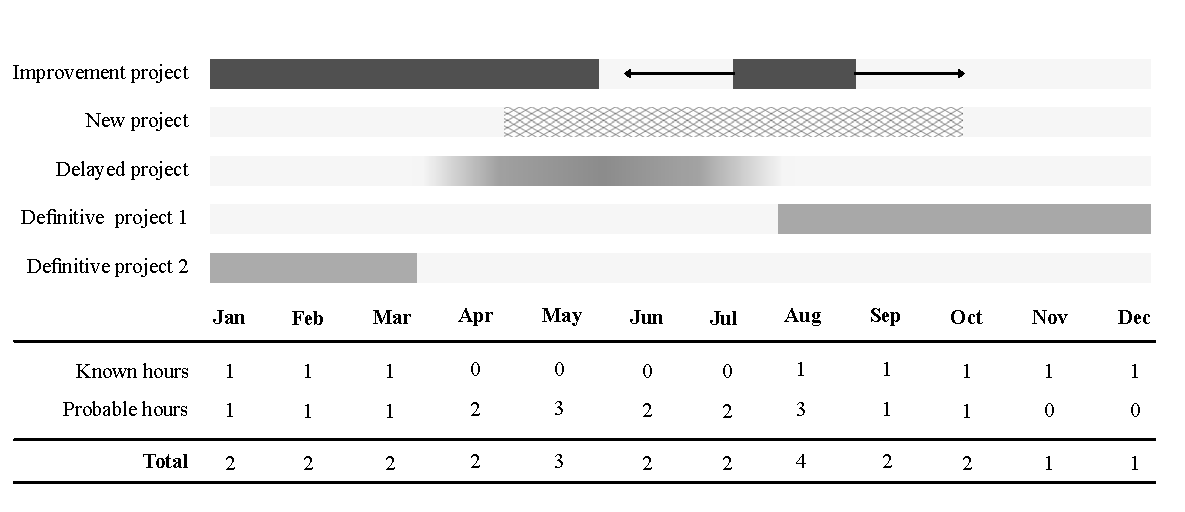
\includegraphics[width=15cm]{../Images/slice1.pdf}
\caption{An illustrative example of shifting an improvement project out to another time period to capitalise of possible dead time whilst ensuring not to exceed the given resource capacity.}
\end{figure}

Th objective of this paper is to propose a multi-objective stochastic optimisation model which optimises both the resource utilisation and minimises the risk of over-utilisation. The proceeding chapter provides a literature review on multi-objective stochastic modelling methods. The model formulation is then present in which a deterministic equivalent is proposed and later evaluated using an unnamed company as a test case. Finally the model is evaluated and a conclusion is presented.


\section{Literature review}
This section reviews the literature first on similar problems and second on the chosen methodology. The identified problem falls into both resource allocation and yield management categories which are explored in the context of the hotel and airline industry \citep{cleophas2017resilient}. The problem deals both with conflicting objectives and uncertain constraints and thus multi-objective stochastic optimisation methods shall be reviewed.

\subsection{Contextual applications}

The principle of selling discounted projects to increase the utilisation of the resource pool and thus cover fixed costs is prominent in the hotel industry \citep{badinelli2000optimal}. Similarly, hotels will offer rooms at a discounted rate to ensure the fixed cost of operating the hotel is covered. However, if a room is offered at a discounted rate in the present, the room will not be available at full price in the future. Given the stochastic nature of customer demand, this could lead to either overbooking or under-booking a room \citep{kimes1989basics}.

 \cite{schaefer2005airline} developed a stochastic optimisation problem to determine when a room should be booked out at a discounted rate. The methodology is based on the work of \cite{de1999stochastic} in which the stochastic demand is decomposed into a limited set of realisations and then used to constrain the number of bookings to a cost class. The objective function aims at maximising the number of bookings for each cost class. The final artefact was incorporated into a rolling time horizon to determine an optimal booking policy.
 
Further research has been conducted on booking policies namely and most prominently, in the airline industry. Airplanes incur a fixed cost when traveling between destinations and so planners must ensure that the airplane is at its optimal capacity. Similar to the hotel industry, airlines must determine how many tickets to discount to maximise the utilisation of their fleet \citep{smith1992yield}. 

\cite{subramanian1999airline} developed a dynamic programming model to allocate seats on a oneway flight with multiple cost classes whilst allowing for cancelations, over bookings and absent passengers. The model defines a recursion function that selects one of three possible events to maximise the total revue namely, a request for a seat, cancellation of seat or a null event with each seat associated to a cost class. 

\subsection{Methodologies}
As made evident by the reviewed literature, such a problem must maximise the use of an asset whilst mitigating the risk of reduced profit. Thus, the chosen methodology must be able to resolve conflicting objectives under uncertainty. \cite{rardin1998optimization} provides several methods for solving multi-objective optimisation problems which include lexicographic or pre-emptive optimisation, weighted sum optimisation and goal programming.

In lexicographic optimisation, multiple objectives are optimisation by considering one objective at a time. Once a solution is obtained, it is imposed as a constraint for the proceeding objectives. One advantage is that lexicographic optimisation generates efficient solutions. However, in cases where alternative optima are rare lexicographic optimisation severely restricts the solutions space. 
To reduce the restrictive constraints imposed by sequential objectives, the weighted sum approach can be used. In this approach, multi-objectives are combined into a single composite function and assigned specific weights. Objectives with positive weights are maximise and negative weights minimise. Solutions generated by this approach are all efficient. A critic against this approach is evaluating the weighting critical which is qualitatively evaluated.

Determining a weighting for an objective is abstract and lacks relevance to decision makers who typically set targets or goals for certain objectives. The goal programming approach supports this practical consideration as it is aims to minimise the deviation from the target level rather than maximise or minimise quantities. Adjustments to this formulation must be made to ensure an efficient solution.

Goal programming can be used in conjunction with other methods to solve stochastic optimisation problems. A simple approach makes used of an expected value approximation \citep{kall1994stochastic}. The random variable is estimated using an appropriate summary static such as the mean or median. These models do not encapsulate the stochastic nature of the system and may in practice lead to sub-optimal solutions.

\cite{nemirovski2006scenario} proposed the scenario approach which generates $N$ constraints or scenarios for all random variables to ensure an optimal solution. The number of scenarios, $N$, is estimated using a formula which ensures that the solution is optimal given a certain confidence interval. This approach accommodates for the stochasticity of the random variable but may overly constrain the model and increase computational complexity as the the number of constraints increase with the number of random variables and the size of the confidence interval. To reduce the number of constraints an analytical approach which essentially estimates a single constraint and is independent of the size of the confidence interval. However, the random variable must be rotationally invariant for this method to be applied.

From the reviewed literature is has been determined that goal programming accompanied by the scenario approach may serve as viable solution approaches. Goal programming provides a relevant and practical approach for addressing the multiple approaches


\section{Model formulation and solution approach}
As with the airline and hotel industry, consulting firms must determine an optimal project schedule by allocating discounted improvement projects within a period, given the uncertainty of other projects. In this section a stochastic optimisation is formulated using gaol programming and is then decomposed into a deterministic equivalent. 

\subsection{Stochastic formulation}
The stochastic formulation of the optimisation problem requires that random variables be explicit noted and expressed as uncertain. The following formulation is proposed. 
\vspace{12pt}

\begin{tabular}{ll}
$x_{t}\triangleq$ & number of hours allocated to improvement project for month $t$, where $t \in T$\\
$\tilde{s}_{jt} \triangleq$&  random variable indicating the number of hours allocated to project $j$ in \\
& month $t$, where $j\in J$\\
$r_t \triangleq$ & availability of resource pool in hours for month $t$ \\
%$q_i \triangleq$& required hours for improvement project $i$ \\
%$u_j \triangleq$& required hours for scheduled project $j$ \\
\end{tabular}

\vspace{12pt}

The random variable $\tilde{s}_{jt}$ comprises of $\zeta_b, \forall b \in B$, implying that each project $j$ can have at most a single random variable. Projects that have been scheduled with certainty are constant i.e. for $t\in \{1,\dots ,5\}$ and $i\in \{1,2,3\}$

\begin{equation}
	\tilde{s}_{jt} = \begin{bmatrix}
		0 & \zeta_1 & \zeta_1 & \zeta_1 & 0 \\
		160 & 160 & 160 & \zeta_2 & \zeta_2 \\
		0 & 320 & 320 & 320 &0
	\end{bmatrix}
\end{equation}

In this instance, project 1 is potential project, project 2 may be delayed and project 3 is known with certainty to begin at the set time. A single resource can generate up to 8 hours in a single day. The formulation of $\tilde{s}_{jt}$ is context specific and is must be applied to a specific use case.

Following the goal seek programming approach, the utilisation maximisation and risk minimisation objectives are abstracted into two deficiency variables, namely $d_1$ and $d_2$ respectively. To ensure the solution is efficient $\epsilon = 0.0001$ is defined and the variables from the constraints below are included in the objective function resulting in the following objective function.

\begin{equation}
	\min z = d_1 + d_2 - \epsilon \bigg{(} \sum_{t=1}^T x_{t}\big{(}\frac{1}{r_t}+1 \big{)} \bigg{)}
\end{equation}

Subject to

\begin{align}
	\label{eq.cont1}
	\sum_{t=1}^T\sum_{j=1}^J \frac{x_{t}+\tilde{s}_{jt}}{r_t} +d_1 \geq 0.8  \\ 
	\label{eq.cont2}
	x_{t} + \sum_{j=1}^J \tilde{s}_{jt} -d_2\leq r_t && \forall t \in T \\
	x_{it} \geq 0 &&  \forall t \in T \\
		d_1,d_2 \geq 0
\end{align}
Constraint \ref{eq.cont1} ensures that the resource utilisation as a percentage is at least 80\% and penalises the objective function if the utilisation is below the goal. Constraint \ref{eq.cont2} ensures that the total resource utilisation stays below the maximum capacity and if the maximum capacity is surpassed, the objective function is penalised.

\subsection{Deterministic equivalent}
To solve the optimisation problem a deterministic equivalent must be formulated. 
Constraint~\ref{eq.cont1} and \ref{eq.cont2} are applicable for 80\% of the time \citep{nemirovski2006scenario}. To accommodate this requirement, the constraint is expressed as
 \begin{align}
 \label{eq:det1}
	P\bigg{(}\sum_{t=1}^T\sum_{j=1}^J \frac{x_{t}+\tilde{s}_{jt}}{r_t} +d_1 \geq 0.8\bigg{)} \geq 0.8  \\ 
	 \label{eq:det2}
	P\bigg{(} x_{t} + \sum_{j=1}^J \tilde{s}_{jt} -d_2\leq r_t\bigg{)} \geq 0.8  && \forall t \in T 
\end{align}
 

where $P$ indicates the probability of this constraint being used. To solve this problem, a set of $N$ constraints must be derived from a random sample of the random variable $\tilde{s}_{jt}$ which will convert equation~\ref{eq:det1} and \ref{eq:det2} into the following form as define by \cite{nemirovski2006scenario}.
\begin{align}
	P\big{(}F(x,\zeta^v)\leq 0 \big{)} \geq 1 - \alpha && v=1,\dots,N
\end{align}

The scenario approach is implemented as follows.

\begin{align}
	P\bigg{(}\sum_{t=1}^T\sum_{j=1}^J \frac{x_{t}+\tilde{s}_{jt}}{r_t} +d_1 \geq 0.8\bigg{)} \geq  1-0.2   \\ 
	P\bigg{(} x_{t} + \sum_{j=1}^J \tilde{s}_{jt} -d_2\leq r_t\bigg{)}\geq  1-0.2
	\label{q1b11}
\end{align}

From this form we can deduce that $\alpha = 0.2$ and $n$ is equivalent to the number of random variables. It is then assumed that a 95\% confidence interval should be applied resulting in a $\delta = 0.05$. The confidence interval ensures that 95\% of the samples will satisfies the constraint 80\% of the time. These values are used to calculate the number of $N$ samples  using the following formula.

\begin{align}
	N=[ 2n\alpha^{-1}\ln(\frac{12}{\alpha}) + 2\alpha^{-1}\ln(\frac{2}{\delta})+2n]
	\label{q1eqN}
\end{align}

The known values are inserted into the formula where $|Q| = N$ is the sample set, reformulating the constraints as 

\begin{align}
 x_{t} + \sum_{j=1}^J s_{jt}^{q} -d_2\leq r_t && \forall t \in T,\forall q\in Q \\
\sum_{t=1}^T\sum_{j=1}^J \frac{x_{t}+s^q_{jt}}{r_t} +d_1 \geq 0.8  
\end{align}



The model is then solved in \texttt{R} using the \texttt{LpSolve} package.


\section{Numerical example}

\begin{table}[]
\centering
\caption{The upcoming project schedule for the next 12 months for Firm X.}
\vspace{12pt}
\begin{tabular}{r|cccccccccccc}
\hline
\multicolumn{1}{l}{} & \multicolumn{12}{c}{\textbf{Month}}  \\
\hline            
\multicolumn{1}{l}{} & 1 & 2 & 3 & 4 & 5 & 6 & 7 & 8 & 9 & 10 & 11 & 12 \\
\hline 
\textbf{Project 1}   & 220 & 160 & 160 & 320 & 320 & 160 & 80 & 80 & 60 & 60  & 60  & 0  \\
\textbf{Project 2}   & 80 & 80 & 80 & 160 & 160 & $\zeta_1$ & $\zeta_1$ & 0 & 0 & 0  & 0  & 0  \\
\textbf{Project 3}   & 0 & 0 & 0 & 0 & 0 & $\zeta_2$ & $\zeta_2$ & $\zeta_2$ & $\zeta_2$ & $\zeta_2$  & $\zeta_2$  & $\zeta_2$  \\
\textbf{Project 4}   & $\zeta_3$ & $\zeta_3$ & $\zeta_3$ & $\zeta_3$ & $\zeta_3$ & $\zeta_3$ & $\zeta_3$ & $\zeta_3$ & $\zeta_3$ & $\zeta_3$ & $\zeta_3$  & $\zeta_3$  \\
\textbf{Project 5}   & 0 & 0 & 0 & 0 & 0 & $\zeta_4$ & $\zeta_4$ & 250 & 250 & 250  & 200  & 0 \\
\hline
\end{tabular}
\label{tab:projects}
\end{table}

This section considers a numerical example of improvement project scheduling given uncertainty. The purpose of this example is to illustrate the functionality of the model formulation. The formulated model is applied to an anonymous consulting firm referred to as \textbf{Firm X}. Firm X specialises in enterprise system implementations and has a total of 5 resources available, setting $r_t=800 \forall t\in T$. Table~\ref{tab:projects} illustrates the 12 month project forecast estimated by project managers at Firm X 

\begin{align}
	\zeta_b = \{U(50,75),U(250,300),U(100,150),U(50,100)\} && b\in \{1,\dots,4\}
\end{align}

 where $\zeta_b$ is uniformly distributed. Finally, the number of scenarios as defined by \cite{nemirovski2006scenario} is estimated using the formula below
\begin{align}
	N=&[ 2(4)(0.2)^{-1}\ln(\frac{12}{(0.2)}) + 2(0.2)^{-1}\ln(\frac{2}{(0.05)})+2(2)] \\
	\label{q1eqN}
		N=&252
\end{align}

This implies that 252 random samples of each constraint will be used to solve the problem. As this model considers multiple objectives namely, maximising utilisation and minimising the risk of over-utilisation it, it is important to recall that all solutions generated by the adjusted goal seek programme are efficient. This implies that one objective cannot be improved upon without degrading the other. The model is abstracted in \texttt{R} and returns the following results.

\begin{align}
	\max z &= -0.000250\\
	x_t &= \{350, 410, 410, 170, 170,  31, 111,  22,  42,  42,  92, 650\}\\
	d_1 &= 0 \\
	d_2 &= 0 \\
\end{align}

Figure~\ref{fig:2} illustrates the average utilisation across all projects which is well exceeds the target goal of 0.8. In several instances the utilisation maxes out at 1.0 however the model does not schedules more improvement projects than required.

\begin{figure}[]
\label{fig:2}
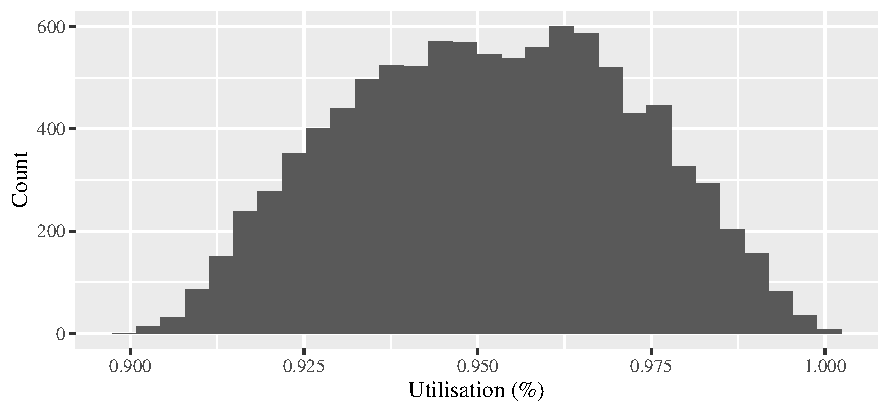
\includegraphics[width=15cm]{../Images/GGplotOverview}
\caption{The overall utilisation the random variable $\zeta_b$ representing the possible and known hours required for each project was sampled 1000 times. For each sample the hours used by each project were totalled, subtracted from the proposed solution and divided by the available hours. These values where averaged to generate this histogram.}
\end{figure}


\section{Model evaluation}
In this section a sensitivity analysis is conducted to evaluate the impact of varying parameters namely, the resource pool size.
As depicted in Figure~\ref{fig:3}, the average utilisation distribution increasingly shifts 27.32\% when the resource pool is reduced by 25\% or 200 hours.However, with an increase of 200\% or 800 hours the shift decreases to mere 2.52\% increase. This implies that the model will schedule as many hours as available to improvement projects, which would increase utilisation and still mitigate the risk of over-committing to projects. 

Maintaining the new resource pool level of 1600 hours, the model is run again however the variation in $\zeta_b$ is increased to  

\begin{align}
	\zeta_b = \{U(50,200),U(100,350),U(100,300),U(50,300)\} && b\in \{1,\dots,4\}
\end{align}

The results do not significantly differ from that of the base case with a decreasing shift of 5.25\%. Thus the model is sensitive to lowering of the resource pool.

\begin{figure}[]
\label{fig:3}
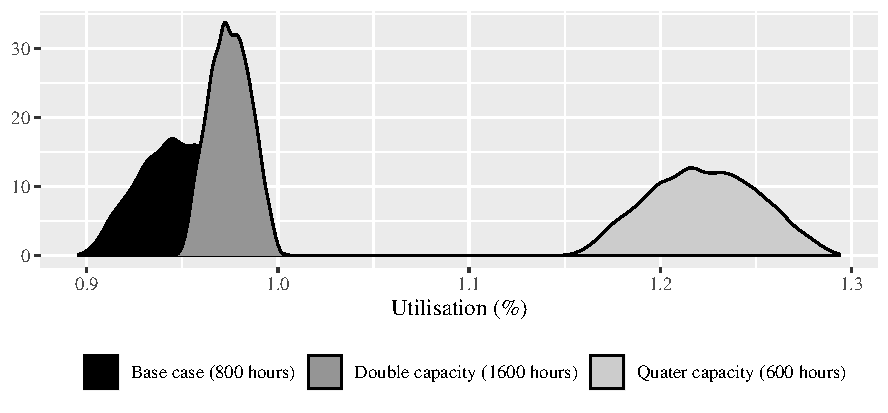
\includegraphics[width=15cm]{../Images/ggsens}
\caption{The average utilisation distribution as a density plot of three cases namely; the base case of 800 available hours, the double capacity case of 1600 hours (double capacity) and the quarter capacity case in which the resource pool was reduced by 200 hours.}
\end{figure}





\section{Conclusion}
The consulting industry is filled with operational challenges that have the potential to end a business. With careful planning, consulting firms can ensure a consistent stream of revenue to cover the fixed cost of specialised labour. Various management techniques such as yield management or revenue management offer various qualitative tools to achieve this, however to successfully implement such techniques often requires concerted mental effort. Deploying a quantitate approach can assist in routine decision making, reducing the effort for managers to apply themselves elsewhere. 

The objective of this study was to create a multi-objective scheduling model under uncertainty to assist decision makers in consulting firms in determining periods in which discounted improvement project may be offered to customers. The model successfully schedules improvement projects, increasing utilisation of the resource pool whilst mitigating the risk of over-committing to possible projects. 

Future improvements should incorporate the various cost classes for improvement projects, including a third objective of maximising revue. Such an inclusion would permit decision makers to further constrain the model, reducing the hours allocated to discounted improvement projects which could be allocated to fully priced projects. It should be noted that to validate such a model would require an assessment against actual results.


\bibliography{Bib}
\addcontentsline{toc}{section}{References}
\newpage
\section*{Appendix: R Script}

\begin{verbatim}
	---
title: "R Notebook"
output: html_notebook
---
#Library import
```{r}
library(tidyverse)
library(lpSolve)
```
#Custom function
```{r}
#Generate list of 0 and 1 for constraint creation
matMaker <- function(ones,len){
  temp <- rep(0,len)
  temp[ones] <- 1
  return(temp)
}

set.seed(123123)
```



# Pre-calculations
The following code evaluates the number of scenarios to be generated
```{r}
N_Prob_FN <- function(n,a,z){
  return(2*n*a^-1*log(12/a)+2*a^-1*log(2/z)+2*n)
}

N <- round(N_Prob_FN(n = 5, a = 0.2, z = 0.05),0)
N
```


# Random constraint function 
When called, this function will generate a random instance of s_jt
```{r}
fn.s_jt <- function(){
  
z1 <- round(runif(1,50,75),0)
z2 <- round(runif(1,250,300),0)
z3 <- round(runif(1,100,150),0)
z4 <- round(runif(1,50,100),0)

          # time t ->
s_jt<- c(220,160,160,320,320,160,80,80,60,60,60,0, 
          80,80,80,160,160,z1,z1,0,0,0,0,0,           
          0,0,0,0,0,z2,z2,z2,z2,z2,z2,z2,
          z3,z3,z3,z3,z3,z3,z3,z3,z3,z3,z3,z3,
          0,0,0,0,0,z4,z4,250,250,250,200,0
          )

return(s_jt)
}

fn.s_jt()



```



# Varibale definition

```{r}
t <- 12
j <- 5
r <- 800
e <- 0.0000001

obj.xt <- e*(r^(-1) +1)

#        d1, d2, x1 -> x12
obj <- c(1,1,-rep(obj.xt,12))

const1.lhs.q <- data.frame()
const1.rhs.q <- data.frame()
const2.lhs.q <- data.frame()
const2.rhs.q <- data.frame()

const1.eql <- rep("<=", N*t) %>% matrix(byrow = TRUE, ncol = 1)
const2.eql <- rep(">=",N) %>% matrix(byrow = TRUE, ncol = 1)

for ( i in 1:N){
  
  const.random <- fn.s_jt() # for each q Zb changes, not for each constraint 
  
  const1.lhs <- cbind(rep(0,t),rep(-1,t),diag(t))
  const1.rhs <- r-c(sum(matMaker(ones = seq(1, to = t*j, by = 12),len = t*j)*const.random),
                sum(matMaker(ones = seq(2, to = t*j, by = 12),len = t*j)*const.random),
                sum(matMaker(ones = seq(3, to = t*j, by = 12),len = t*j)*const.random),
                sum(matMaker(ones = seq(4, to = t*j, by = 12),len = t*j)*const.random),
                sum(matMaker(ones = seq(5, to = t*j, by = 12),len = t*j)*const.random),
                sum(matMaker(ones = seq(6, to = t*j, by = 12),len = t*j)*const.random),
                sum(matMaker(ones = seq(7, to = t*j, by = 12),len = t*j)*const.random),
                sum(matMaker(ones = seq(8, to = t*j, by = 12),len = t*j)*const.random),
                sum(matMaker(ones = seq(9, to = t*j, by = 12),len = t*j)*const.random),
                sum(matMaker(ones = seq(10, to = t*j, by = 12),len = t*j)*const.random),
                sum(matMaker(ones = seq(11, to = t*j, by = 12),len = t*j)*const.random),
                sum(matMaker(ones = seq(12, to = t*j, by = 12),len = t*j)*const.random)) %>% matrix(byrow = TRUE, nrow = t)
  

  const2.lhs <- c(1,0,rep(1,12)/r)

  
  const2.rhs <- 0.8 - sum(const.random/(r*t*j))
  
  
  const1.lhs.q <- rbind(const1.lhs.q, const1.lhs) %>% as.matrix()
  const1.rhs.q <- rbind(const1.rhs.q, const1.rhs) %>% as.matrix()
  const2.lhs.q <- rbind(const2.lhs.q, const2.lhs) %>% as.matrix()
  const2.rhs.q <- rbind(const2.rhs.q, const2.rhs) %>% as.matrix()
}


#const1.lhs.q
#const1.rhs.q
#const2.lhs.q
#const2.rhs.q

const.lhs <- rbind(const1.lhs.q,const2.lhs.q)
const.rhs <- rbind(const1.rhs.q,const2.rhs.q)
const.eql <- rbind(const1.eql,const2.eql)

lp <- lp(direction = "min", 
   objective.in = obj, 
   const.mat = const.lhs, 
   const.dir = const.eql, 
   const.rhs = const.rhs)

lp

lp$solution %>% round(digits = 2)


```

# Solving the linear programme
```{r}

var.Utilisation <- c()
  
  
for (i in 1:10000){
  var.Utilisation[i] <- mean((matrix(data = fn.s_jt(),byrow = TRUE, ncol = 12)%>% colSums() + lp$solution[3:14])/r)
}

gg.overviewPlot <- var.Utilisation %>% as.data.frame %>% ggplot(aes(x = var.Utilisation))+geom_histogram()+
  labs(x = "Utilisation (%)", y = "Count")+
  theme_gray(base_size = 11, base_family = "serif")+
  theme(legend.title=element_blank(), legend.position="bottom")+
  scale_fill_grey(start = 0, end = 0.7)

 ggsave(plot = gg.overviewPlot, device = "pdf", filename = "../Images/GGplotOverview.pdf", units = "cm", width = 15.056, height = 7)

```






\end{verbatim}

\end{document}

